%mainfile: ../../master.tex
\section{Use Cases}\label{sub:usecases}

This section will describe ways of interacting with the prototypical system derived from the requirements. The rich picture \cref{fig:richpicture}, show the general exchange of information within the problem domain. This is useful for developing an overview of different actors interacting in the problem domain.

\begin{figure}
  \centering
  \begin{adjustbox}{max width=\textwidth}
    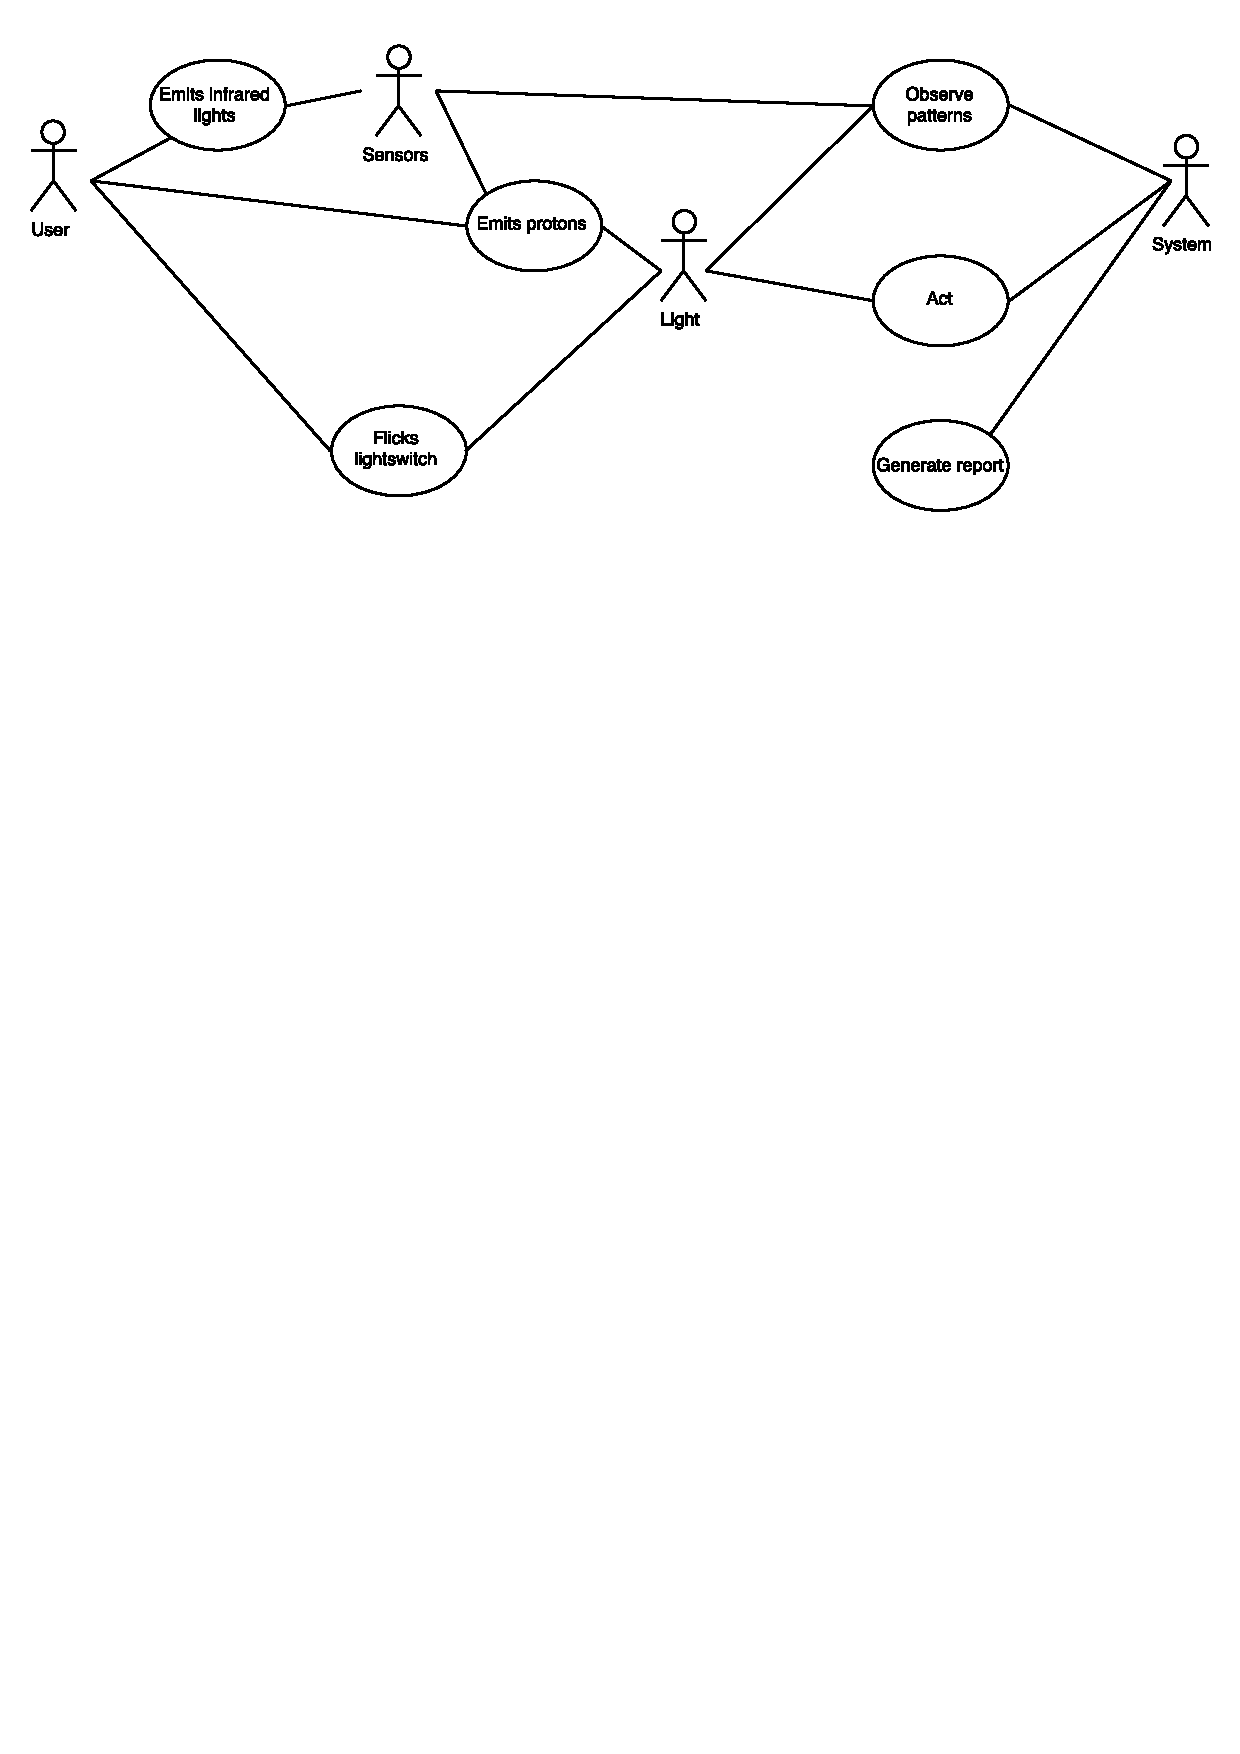
\includegraphics{Usecases.pdf}
  \end{adjustbox}
  \caption[Rich picture]{Rich picture of the problem domain}
  \label{fig:richpicture}
\end{figure}

\subsection{Problems with multiple users}
There are several concerns regarding multiple users of the system, as the system cannot differentiate persons. These concerns will be described in the following sections.

\subsubsection{Differing Usage Patterns}
Different users' usage patterns most likely differ, which could result in the system applying its knowledge of a user's usage pattern on the wrong user, thereby performing a wrong action.
\paragraph{Example}
Consider two persons, A and B. A and B live in the same home, using the same home automation system. When A arrives home, the first thing A does is turn on the light in the hallway and the turn on the TV. B has a very irregular behaviour pattern when arriving home. After some time, the system learns A's usage pattern, that is, after a person arrives home, the light in the hallway should be turned on, and then the TV should be turned on. As the system is not able to differentiate persons, B arrives home one day, and then the system turns on the light in the hallway and the TV. This would likely be a wrong action, as the learned pattern regards another person.
\subsubsection{Interfering Usage Patterns}
Different users' usage patterns may be similar, yet slightly different. This could result in the system never learning the patterns of any of the users, due to the system considering the two patterns as one, because of identical preconditions.
\paragraph{Example}
Consider two persons, A and B. A and B live in the same home, using the same home automation system. When A arrives home, A turns on the light in the hallway and then turns on the TV. When B arrives home, B turns on the light in the hallway and then turns on the radio. As the system is not able to differentiate the two, it will never be able to learn a meaningful pattern, as it will not be able to decide whether to turn on the TV or turn on the radio.